\documentclass[tikz,border=6pt]{standalone}
\usetikzlibrary{arrows.meta, positioning}

\begin{document}
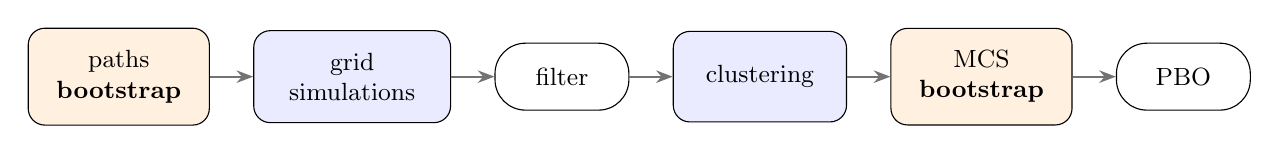
\begin{tikzpicture}[
    box/.style={draw, rounded corners=6pt, align=center, minimum height=1.15cm, inner sep=8pt, font=\small},
    pill/.style={draw, rounded corners=11pt, align=center, minimum height=0.85cm, minimum width=1.7cm, inner sep=6pt, font=\small},
    arr/.style={-{Stealth[length=6pt]}, thick, black!55},
    node distance=0.55cm
  ]

  \node[box, fill=orange!12, minimum width=2.3cm] (paths) {paths \\ \textbf{bootstrap}};
  \node[box, fill=blue!8, minimum width=2.5cm, right=of paths] (grid) {grid \\ simulations};
  \node[pill, right=of grid] (filter) {filter};
  \node[box, fill=blue!8, minimum width=2.2cm, right=of filter] (cluster) {clustering};
  \node[box, fill=orange!12, minimum width=2.3cm, right=of cluster] (mcs) {MCS \\ \textbf{bootstrap}};
  \node[pill, right=of mcs] (pbo) {PBO};

  \draw[arr] (paths) -- (grid);
  \draw[arr] (grid) -- (filter);
  \draw[arr] (filter) -- (cluster);
  \draw[arr] (cluster) -- (mcs);
  \draw[arr] (mcs) -- (pbo);
\end{tikzpicture}
\end{document}
